\chapter{Related Works}

\section{Outline}

\begin{outline}
    \1 Short-read sequencing
        \2 Sequencing errors
    \1 Assembler Architecture
        \2 \dBG
        \2 Pre-processing of reads
            \3 \kmer counting \& filtering
                \4 khmer\cite{Zhang2014}
    \1 Navigational Data Structures (NDS)
        \2 \cite{Chikhi2014}
    \1 \emph{FastEtch} \cite{Ghosh2019}
        \2 Online counting $\rightarrow$ Filtering $\rightarrow$ Construction of \dBG
\end{outline}

\section{Notation}

Throughout this work, we use lower-case symbols, such as $t$ and $c$, to represent scalar values. Uppercase symbols, such as $\strname{X}$ and $\strname{Y}$, represent strings. Finally, calligraphic uppercase symbols, such as $\readset$, are used to represent sets. Strings and sets are $0$-indexed, and the notation $X[i:j]$ represents the substring of $X$ from position $i$ up to, but not including, position $j$. When used between two string, or a string and a character, $\strname{X} \cdot \strname{Y}$ represents the concatenation of $\strname{X}$ and $\strname{Y}$.

\section{\dBG{s}}
\label{sec:dBG}

% - Detailed explanation of \dBG of a set of DNA sequences
%   - reverse complements
% - How it is going to be used
% - Operations
%   - Insert node
%   - Insert edge
%   - Query node
%   - Query edge / star 
% - Space-efficient representations - that's what we propose

The \keyterm{\dBG of order $k$} of a string \strdef{x}{n}, $G(X;k)=(V,E)$, is defined as the directed graph whose nodes $V$ represent all distinct \kmer{s} (i.e. substrings of length $k$) of \strname{X}, and such that any two nodes representing $(k-1)$-overlapping \kmer{s} are connected by an edge labeled by the last character of the second \kmer. For example if $k=3$ and $X$ contains the substring \chr{ACGT} then the consecutive triplets \chr{ACG} and \chr{CGT} will originate the edge $\chr{ACG}\stackrel{\chr{C}}{\longrightarrow}\chr{CGT}$. Hence the edges $E$ represent all distinct $(k+1)$-mers of $X$. 
% That is, given two nodes on the graph, they each represent a distinct sequence of symbols $S_1$ and $S_2$, and there is an edge between them if and only if the tail of $S_1$ is the head of $S_2$.

In genome sequencing, \dB graphs are used in the assembly process to represent the distinct \kmer{s} in a set \readset of randomly distributed fragments of the source DNA \strname{S}, called \keyterm{reads}, generated by the sequencing machines. The amount and total length of the reads is determined by the \keyterm{coverage} of the sequencing process, i.e. the number of times \strname{S} was cloned and sequenced. Ideally, \strname{S} could be obtained from an Eulerian traversal of $G(\readset, k)$. Unfortunately however, due to sequencing errors and repeats, such a straightforward approach is not feasible, but the \dBG can still be used to produce a collection of partial assemblies, called \keyterm{contigs}, which can then be further combined to form the original genome \cite{Pevzner2001}. Figure~\ref{fig:dbgexample} presents an example of the \dBG in this context.

\begin{figure}[htbp]
	\begin{center}
    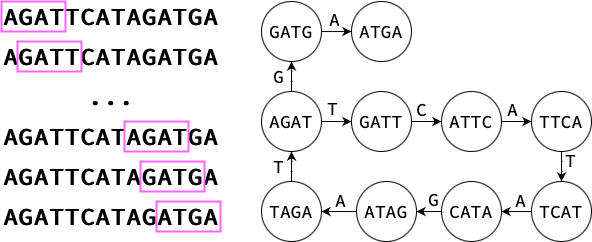
\includegraphics[width=0.8\textwidth]{figures/dbg-example}
	\end{center}
	\caption{Example of a \dBG. $k=4$}\label{fig:dbgexample}
\end{figure}

\subsection{Reverse Complements}
\label{subsec:dBG-reversecomplements}

One difficulty of using \dBG{s} to represent DNA data is the presence of \keyterm{reverse complements}. When generating sequencing reads, the machine reads either of the two complementary strands of a fragment of the input DNA. That is, the output read may correspond to the sequence \strname{S} in the forward (5'-3') direction, or its reverse complement \strname{\overline{S}} in the backward (3'-5') direction, with
\strname{\overline{S}} being obtained from \strname{S} by swapping each base with its Watson-Crick complement
($\A \leftrightarrow \T$, $\C \leftrightarrow \G$) and then reversing the string, and vice versa. For example, the reverse complement of the sequence $S=\chr{AGTACGGTC}$ is $\overline{S}=\chr{GACCGTACT}$ and vice versa.

To deal with reverse complements, reads are processed twice, once in each direction. Nodes representing \kmer{s} that are reverse complements of each other are merged, with edges made bidirectional. Alternatively, those nodes can be kept distinct, resulting in a symmetric graph in which, as noted by Conway \& Bromage, ``a forward traversal corresponds to the backwards traversal on the reverse complement path, and vice versa.'' \cite{Conway2011}
% As in \cite{Conway2011}, this will be treated by processing
% all reads in both directions, without, however, merging nodes representing reverse complements. As noted by Conway \& Bromage: ``This
% makes the graph symmetric; a forward traversal corresponds to a backwards traversal on the reverse complement path, and vice versa.``
% \cite{Conway2011}

\subsection{Selecting the \kmer{s} for the \dBG}
\label{subsec:dBG-selectingkmers}

Another difficulty of using a \dBG to represent DNA data is dealing with sequencing errors. During the sequencing process, there is a small error rate associated with reading any base from \strname{S} (0.1\%--1\% per base in Illumina \cite{Metzker2010}). As a result, many of the \kmer{s} extracted from the reads in \readset are erroneous. As discussed by Conway \& Bromage, this causes the number of spurious \kmer{s} to grow proportionally to the number of bases in the reads $|\readset|=\sum_{\strname{X}_i \in \readset} |\strname{X}_i|$, determined by the coverage, while the number of true \kmer{s} is proportional to the size of the genome $|\strname{S}|$ \cite{Conway2011}.

Although modern sequencing machines generate a quality score associated with each base, it is not possible to know exactly what parts of the reads are erroneous, and so we cannot tell whether a \kmer should be added to the \dBG without more information. However, real \kmer{s} are expected to appear a number of times close to the sequencing coverage $c$, or a multiple of $c$ in case of repeats, whereas spurious \kmer{s} resulting from sequencing errors are commonly low-frequency or even unique \cite{Conway2011, Zhang2014, Ghosh2019}. As such, a natural way of filtering the \kmer{s} obtained from the reads is to discard those that have a low frequency. Hence we consider a \kmer to be a real \kmer iff it occurs more than some threshold $t$, in which case added to the \dBG.

Counting \kmer{s} in a set of reads in a time- and space-efficient manner is, in itself, a challenging task, which is commonly performed as a preprocessing step to the \dBG construction \cite{Zhang2014}. Some assemblers, however, introduce \kmer counting as a part of the \dBG construction, such as the \emph{FastEtch} assembler, which uses a \cm sketch (discussed in Section~\ref{sec:countmin}) to do so \cite{Ghosh2019}.

\subsection{\dBG representation}
\label{subsec:dBG-representation}

A \dBG can be represented either by its set of nodes (\kmer{s}) or edges ($(k+1)$-mers) equivalently, as one can be derived from the other. Therefore, a structure that can determine if a given node $x$ is a member of $G$ can represent the \dBG. Conway \& Bromage showed that the lower bound on the space required to \emph{exactly} represent these \keyterm{membership data structures} (MDS's) is $\Omega(n \log n)$, with $n=|V(G)|$ \cite{Conway2011}.

In order to further improve space-efficiency, new representations were created that trade deterministic exactness for a probabilistic approach. Pel \emph{et al.} showed that a probabilistic representation based on a Bloom Filter could accuratly represent a \dBG with as little as 4~bits per \kmer \cite{Pell2012}.

However, Bowe \emph{et al.} \cite{Bowe2012} and Chikhi \& Rizk \cite{Chikhi2013} independently observed that giving up deterministic exactness isn't the only option for obtaining better space-efficiency, introducing two new representations that use $O(n)$ and $O(n \log k)$ bits, respectively, and allow for an exact traversal of the \dBG from a starting set of known member nodes. This is possible due to the fact that a \dBG is not queried for membership of random nodes, but rather for potential neighbors of nodes already known to be in the graph. As such, the structures designed by the two groups do not offer a deterministically exact membership query operation, instead offering a neighborhood query operation that is exact for the members of the graph \cite{Bowe2012, Chikhi2013}. Chikhi \emph{et al.} later named this new form of representation a \keyterm{Navigational Data Structure} (NDS) and showed that the lower bound on the number of bits required to exactly represent a \dBG with an NDS is $3.24n$ \cite{Chikhi2014}.

Beyond the distinction between probabilistic and exact, and MDSs and NDSs, there is also a distinction between \keyterm{static} and \keyterm{dynamic} representations for \dBG. Static representations are constructed once and never altered, whereas dynamic representations support operations such as insertion and deletion of nodes, useful in population-scale studies due to their everchanging nature \cite{Alipanahi2021}.

% A \dBG can be represented either by its set of nodes (\kmers) or edges ($(k+1)$-mers) equivalently, as one can be derived from the other.
% As such, a structure that can answer queries about the presence of a given node on the graph is enough to
% represent the graph. Conway\&Bromage showed that the lower bound on the space required to
% \emph{exactly} represent a \dBG is $\Omega(n \log n)$ bits, where $n$ is the number of nodes\remove[isn't this obvious?]{,
% and $4^k > n$}\cite{Conway2011}.

% \asq{Isso precisa ser reescrito: NDSs não são necessariamente representações probabilisticas. Elas apenas substituem a consulta de presença de um nó pela consulta de vizinhança.}

% In order to further improve space-efficiency, new representations were created that trade deterministic exactness for a probabilistic approach. For instance, the so-called \keyterm{Navigational Data Structures} (NDS) have some probability of giving an erroneous answer to a membership query, 
% but can still be used to navigate the graph \cite{Chikhi2014}. This \change{definition is useful}{is} due to the fact that a \dBG is usually not queried for membership of \change{randomly selected}{random} nodes, but rather \remove{only} potential neighbors of \change{a known member node is queried}{nodes already known to be in the graph}. In the same paper where they introduce
% the idea of NDS \cite{Chikhi2014}\paguso{correct?}\asq{Esse artigo de Chikhi \emph{et al.} é a introdução e formalização do conceito de NDSs em oposição às Membership Data Structures. Em segunda leitura, porém, categorizar nossas estruturas como NDSs é incorreto porque NDSs devem dar respostas exatas para consultas de vizinhança, o que nós não garantimos.}, Chikhi \emph{et al.} also present a lower bound for the number of bits needed to represent such a structure as $3.24n$.
% In sections \ref{sec:debruijncountmin} and \ref{sec:debruijnhashtable} we will introduce two new NDS's. \asq{É necessário reiterar
% os objetivos das duas estrutas aqui, visto que isso já seria feito na introdução e é feito nas próprias sessões dedicadas a cada estrutura?}\paguso{até o momento, acho que não.}

\subsubsection{Operations}
\label{subsubsec:dbg-operations}

Chikhi \emph{et al.} \cite{Chikhi2019} present the following set of operations common to many data structures for representing a \dBG.

\begin{enumerate}
  \item \emph{Construction} of the data structure
  \item \emph{Insertion} of a new \kmer
  \item \emph{Deletion} of an existing \kmer.
  \item \emph{Membership query}: Given a \kmer $X$, returns true iff $X \in G$
  \item \emph{Forward neighbor query}: Given a \kmer $X$ and a base $a$, returns true iff $X[1:k] \cdot a \in G$
  \item \emph{Backward neighbor query}: Given a \kmer $X$ and a base $a$, return true iff $a \cdot X[0:k-1] \in G$.
\end{enumerate}

Note that a representation that implements the \emph{construction} and \emph{membeship query} operation can use those to implement some version of the others (e.g. by reconstructing the graph with the desired insertion or deletion, or by querying for the membership of the desired neighbor). However, dynamic representations implement \emph{insertion} and \emph{deletion} operations that do not require the reconstruction of the graph, while NDSs don't rely on the membership query to establish if a given forward or backward neighbor is represented in the graph. For example, the neighborhood query described by Chikhi \emph{et al.} \cite{Chikhi2014} as defining NDSs can be implemented by performing \emph{forward} and \emph{backward neighbor queries} for all extensions of the given \kmer and then returning only those for which the result was $\mathit{true}$.